\chapter{Metodi iterativi}
Dato un generico sistema lineare
\begin{equation*}
    Ax=b
\end{equation*}
con $A \in \mathbb{R}^{n \times n}$ invertibile, $b \in \mathbb{R}^n$. I metodi
iterativi permettono, partendo da un vettore iniziale $x^{(0)}$, di costruire una
sequenza di soluzioni $x^{(k)}$ che si avvicinano sempre di più alla soluzione
esatta $\stackrel{\sim}{x}$.
\section{Fill-in}
Dal momento che la maggior parte delle volte la matrice $A$ assume dimensioni molto
grandi e spesso si tratta di matrici sparse, allora esse verranno salvate utilizzando
la rappresentazione sparsa.

Nel momento in cui si effettua una decomposizione PALU o di Cholesky è possibile
che le matrici risultanti non siano più sparse, questo fenomeno è chiamato
\textbf{fill-in}. Questo comporta un aumento di complessità spaziale, portando
ad occupare troppa memoria.

I metodi iterativi permettono di risolvere questo problema, perché utilizzando
le operazioni tra matrici, preservano la natura sparsa di esse, quindi non si
incombe nel fenomeno di fill-in. Questo ha un costo, ovvero che $Ax$ è simile
a $b$.
\begin{equation*}
    Ax \sim b
\end{equation*}
\section{Criterio di arresto}
Negli algoritmi iterativi si ha una quantità, chiamata \textbf{tolleranza}, che
identifica quando una soluzione approssimata $x^{(k)}$ è vicina alla soluzione
esatta.

Per misurare questa vicinanza si utilizza la norma tra vettori. Idealmente,
avendo a disposizione la soluzione esatta $\stackrel{\sim}{x}$, si potrebbe
calcolare l'errore relativo tra la soluzione approssimata e quella esatta, e
fermarsi quando l'errore è minore di una certa tolleranza.
\begin{equation}
    \frac{\|x^{(k)}-\stackrel{\sim}{x}\|}{\|\stackrel{\sim}{x}\|} < \texttt{tolleranza}
\end{equation}
Non potendo conoscere la soluzione esatta allora si riscrive la relazione utilizzano
i seguenti metodi di arresto:
\begin{itemize}
    \item \textbf{Incremento tra due iterate}: alla iterazione $k$ si calcola:
          \begin{equation*}
              \frac{\|x^{(k)}-x^{(k-1)}\|}{\|x^{(0)}\|}< \texttt{tolleranza}
          \end{equation*}
          Questo misura quanto le quantità $x^{(k)}$ e $x^{(k-1)}$ differiscono.
          Ci si ferma quando la differenza è al di sotto della tolleranza. Quindi
          questo corrisponde a calcolare l'errore relativo rispetto alla soluzione
          precedente normalizzato rispetto la soluzione iniziale.
    \item \textbf{Residuo scalato}: alla iterazione $k$ si calcola:
          \begin{equation*}
              \frac{\|b- Ax^{(k)}\|}{\|b\|}< \texttt{tolleranza}
          \end{equation*}
          Dove $A$ e $b$ sono la matrice e il vettore dei termini noti del sistema
          che si sta risolvendo. Quindi questo corrisponde a calcolare l'errore
          relativo rispetto alla soluzione precedente normalizzato rispetto la
          soluzione iniziale.
\end{itemize}
Il criterio di arresto basato sull'incremento tra due iterate successive è
successivamente normalizzato rispetto alla soluzione iniziale, mentre il criterio
di arresto basato sul residuo scalato viene normalizzato rispetto al vettore dei
termini noti.
\begin{nota}
    Questi criteri funzionano per qualsiasi norma si vuole utilizzare.
\end{nota}

Analizzando la \textbf{complessità del criterio di arresto basato sull'incremento
    tra due iterate successive}, si può notare che si effettua una sottrazione
tra vettori di dimensione $n$ ($n$ somme ovvero $\mathcal{O}(n)$), la norma ha
una complessità di $\mathcal{O}(n)$ (quindi $2\mathcal{O}(n)$ perché si calcola
due volte) e successivamente si ha $1$ divisione. Il costo totale risulta quindi:
\begin{equation*}
    \mathcal{O}(n^2)+ \mathcal{O}(n)+2\mathcal{O}(n)+1 = \mathcal{O}(n)
\end{equation*}
Per quanto riguarda la \textbf{complessità del criterio di arresto basato
    sul residuo scalato} si hanno delle operazioni più complesse:
\begin{itemize}
    \item prodotto tra matrice e vettore: $\mathcal{O}(n^2)$
    \item somma tra vettori: $\mathcal{O}(n)$
    \item calcolo di due norme: $2\mathcal{O}(n)$
    \item un rapporto: $\mathcal{O}(1)$
\end{itemize}
Il totale risulta essere quindi:
\begin{equation*}
    \mathcal{O}(n^2)+ \mathcal{O}(n)+2\mathcal{O}(n)+1 = \mathcal{O}(n^2)
\end{equation*}
Il costo è maggiore rispetto al primo criterio anche se rimane sempre polinomiale
di grado basso. In aggiunta si può notare che spesso i metodi iterativi calcolano
già la quantità $b-Ax^{(k)}$ per ottenere la soluzione $x^{(k+1)}$, quindi la parte
più onerosa del calcolo del residuo si sposta nel calcolo della soluzione successiva.
\begin{nota}
    Quando si calcola il residuo si calcola una sola volta la norma di $b$, perché
    per tutto l'algoritmo il vettore rimane invariato.
\end{nota}
\begin{nota}
    In aggiunta non è stato tenuto conto che quando calcoliamo i criteri di arresto
    quando facciamo il prodotto matrice-vettore, la matrice è sparsa, quindi
    il prodotto non è $\mathcal{O}(n^2)$ ma una complessità dipendente dalle entrate
    non nulle.
\end{nota}
\section{Generico algoritmo iterativo}
Tutti gli algoritmi iterativi sono identici a meno della metodologia di calcolo
della soluzione $x^{(k)}$.

Un generico algoritmo prende in input:
\begin{itemize}
    \item una matrice $A$
    \item un vettore dei termini noti $b$
    \item una tolleranza \texttt{tolleranza}
    \item eventuali parametri addizionali utili per il calcolo della soluzione
          $k$-esima.
\end{itemize}

Il vettore $x^{(0)}$ di partenza e sotto opportune ipotesi della matrice $A$, la
scelta della soluzione iniziale mantiene invariata la convergenza dell'algoritmo.

Si ha un ciclo while che ha come condizione la verifica del criterio di arresto,
ovvero uno dei criteri specificati precedentemente. Oltre al criterio di arresto
spesso si aggiunge un numero di iterazioni massime perché spesso si rischia di
non poter mai raggiungere la soluzione esatta.

Nell'algoritmo non si effettuano mai operazioni che modificano la matrice $A$,
quindi non si rischierà l'effetto fill-in.
\begin{nota}
    Il numero di iterazioni massime, per alcuni problemi, può essere stabilito
    a priori in base alla dimensione della matrice. In generale si considera
    sempre un numero arbitrariamente alto.
\end{nota}
\begin{algorithm}
    \caption{Algoritmo iterativo generico}
    \begin{algorithmic}
        \Function{AlgoritmoIterativo}{$A,b,\texttt{tolleranza},\texttt{parametri}$}
        \State $x^{(0)} \gets \text{vettore iniziale}$
        \State $k \gets 0$
        \While{$\text{criterio di arresto} \geq \texttt{tolleranza} \land k < \text{numero massimo di iterazioni}$}
        \State $x^{(k+1)} \gets \text{calcola la soluzione } k \text{-esima}$
        \State $k \gets k+1$
        \EndWhile
        \State \Return $x^{(k)}$
        \EndFunction
    \end{algorithmic}
\end{algorithm}
\section{Metodi iterativi stazionari}
Una strategia comune per definire un metodo risolutivo iterativo è tramite la
procedura di \textbf{splitting}. Data una matrice $A \in \mathbb{R}^{n \times n}$,
supponiamo di spezzarla nel seguente modo:
\begin{equation*}
    A=P-N
\end{equation*}
con $P, N \in \mathbb{R}^{n \times n}$. Con questa decomposizione il sistema lineare
si riscrive nel seguente modo:
\begin{equation*}
    Ax = b \iff (P - N)x = b \iff Px = Nx + b \iff x = P^{-1}Nx + P^{-1}b
\end{equation*}
L'ultima uguaglianza suggerisce la procedura iterativa, ovvero partendo da una
soluzione iniziale $x^{(0)} \in \mathbb{R}^n$ possiamo ricavare le soluzioni
successive tramite la seguente formula:
\begin{equation}
    x^{(k + 1)} =  P^{-1}Nx^{(k)} + P^{-1}b
    \label{eq:iterativo_stazionario}
\end{equation}
Tutti i metodi iterativi si basano sul fatto che il calcolo della matrice $P^{-1}$
sia veloce e facile. Se non fosse così allora converrebbe trovare l'inversa di
$A$ al posto di $P$, in modo tale da calcolare $x=A^{-1}b$.

Questi metodi vengono chiamati stazionari perché le matrici $P, N$ non dipendono
dal parametro $k$.
\begin{teorema}[\textbf{Convergenza metodi stazionari}]\label{th:metodi_iterativi}
    Supponiamo che esista una decomposizione di $A=P - N $ (splitting) con $A, P$
    simmetriche e definite positive. Se anche la matrice $2P - A$ è definita
    positiva allora il metodo iterativo definito nell'equazione \ref{eq:iterativo_stazionario}
    converge per ogni valore iniziale $x^{(0)}$ e $|\lambda_{\max}| < 1$. dove
    $\lambda_{\max}$ è l'autovalore di modulo massimo della matrice $P^{-1}N$.
    Inoltre la convergenza è monotona rispetto alle norme $\|\cdot\|_p$
\end{teorema}

Il teorema appena presentato permette di effettuare delle considerazioni importanti
sui metodi iterativi basati su splitting:
\begin{itemize}
    \item Sicurezza nella convergenza a partire da una qualsiasi soluzione sotto
          le ipotesi del teorema.
    \item Monotonia sull'errore, ovvero a ogni passaggio siamo sicuri che la
          soluzione che abbiamo trovato sia migliore di quella precedente.
    \item Si può utilizzare qualunque norma per calcolare l'errore.
\end{itemize}
Il teorema \ref{th:metodi_iterativi} è complesso da verificare, esiste però Un
diverso teorema che fornisce una condizione necessaria per la convergenza dei
metodi iterativi basati sullo splitting.
\begin{teorema}
    Sia $A$ una matrice a dominanza diagonale allora i metodi che vedremo basati
    sullo splitting convergono
\end{teorema}
Questo assicura che $2P - A$ è definita positiva senza effettuare la decomposizione
si Cholesky che può causare Fill-in.
\begin{nota}
    Matrice a diagonale dominante significa che $|a_{ii}| > \sum_{i \neq j}|a_{ij}|$
\end{nota}
\begin{definizione}
    LA matrice $P^{-1}N$, che solitamente è indicata con $B$, viene chiamata matrice
    di iterazione del metodo.
\end{definizione}
Partendo dall'equazione \ref{eq:iterativo_stazionario} possiamo ricondurci ad
un'espressione simile al residuo scalato nel seguente modo:
\begin{equation*}
    \begin{aligned}
        x^{(k + 1)} & = P^{-1}Nx^{(k)} + P^{-1}b           \\
                    & = P^{-1}(P - A)x^{(k)} + P^{-1}b     \\
                    & = x^{(k)} - P^{-1}Ax^{(k)} + P^{-1}b \\
                    & = x^{(k)} + P^{-1}(b - Ax^{(k)})     \\
                    & = x^{(k)} + P^{-1}r^{(k)}            \\
    \end{aligned}
\end{equation*}
Da questo si evince che $b-Ax^{(k)}$ è il \textbf{residuo} $r^{(k)}$ e questo è
utile se si sta usando il residuo come criterio di stop.
\subsection{Jacobi}
In questo paragrafo introduciamo il metodo iterativo stazionario di Jacobi.
Consideriamo la $i$-esima equazione di un sistema lineare $Ax = b$.
\begin{equation*}
    a_{i1}x_1 + a_{i2}x_2 + \dots + a_{ii}x_i + \dots + a_{in}x_n = b_i
\end{equation*}
se isoliamo la $i$-esima incognita otteniamo:
\begin{equation*}
    x_i = \frac{1}{a_{ii}}(b_i - \sum_{j \neq i}a_{ij}x_j)
\end{equation*}

Vediamo ora come si comporta il metodo di Jacobi. Partiamo dal seguente sistema
lineare:
\begin{equation*}
    \begin{cases}
        a_{11}x_1 + a_{12} x_2 + \dots + a_{1n} x_n= b_1 \\
        a_{21}x_1 + a_{22} x_2 + \dots + a_{2n} x_n= b_2 \\
        \vdots                                           \\
        a_{n1}x_1 + a_{n2} x_2 + \dots + a_{nn} x_n= b_n \\
    \end{cases}\implies
    \begin{cases}
        a_{11}x_1 = b_1 - (a_{12} x_2 + \dots + a_{1n} x_n)                   \\
        a_{22} x_2 = b_2 - (a_{23} x_3\dots + a_{2n} x_n + a_{11}x_1)         \\
        \vdots                                                                \\
        a_{nn} x_n= b_n - (a_{n1}x_1 + a_{n2} x_2 + \dots + a_{nn-1} x_{n-1}) \\
    \end{cases}
\end{equation*}
Per ipotesi dei metodi stazionari, sappiamo che un qualsiasi componente
posizionato sulla diagonale principale della matrice è positivo e diverso da $0$,
quindi possono ottenere il seguente sistema lineare:
\begin{equation*}
    \begin{cases}
        x_1 = \frac{b_1 - (a_{12} x_2 + \dots + a_{1n} x_n)}{ a_{11}}                 \\
        x_2 =\frac{ b_2 - (a_{23} x_3\dots + a_{2n} x_n + a_{11}x_1)}{a_{22}}         \\
        \vdots                                                                        \\
        x_n= \frac{b_n - (a_{n1}x_1 + a_{n2} x_2 + \dots + a_{nn-1} x_{n-1})}{a_{nn}} \\
    \end{cases}
\end{equation*}
Questo può essere visto in modo iterativo:
\begin{equation*}
    \begin{cases}
        x_1^{(k+1)} = \frac{b_1 - (a_{12} x_2^{(k)} + \dots + a_{1n} x_n^{(k)})}{ a_{11}}                       \\
        x_2^{(k+1)} =\frac{ b_2 - (a_{23} x_3^{(k)}\dots + a_{2n} x_n^{(k)} + a_{11}x_1^{(k)})}{a_{22}}         \\
        \vdots                                                                                                  \\
        x_n^{(k+1)}= \frac{b_n - (a_{n1}x_1^{(k)} + a_{n2} x_2^{(k)} + \dots + a_{nn-1} x_{n-1}^{(k)})}{a_{nn}} \\
    \end{cases}
\end{equation*}

Una volta compresa l'idea alla base dell'algoritmo, quello che manca è vedere
i passi sotto forma di uno splitting di matrici. Dobbiamo riprendere i passi per
ottenere lo splitting dei metodi stazionari.
\begin{equation*}
    Ax = b \iff (P - N)x = b \iff Px - Nx = b \iff Px = Nx + b
\end{equation*}
Possiamo ricavare le matrici $P$ e $N$ nel seguente modo:
\begin{equation*}
    P= \left[\begin{array}{cccc}
            a_{11} & 0      & \dots  & 0      \\
            0      & a_{22} & \dots  & 0      \\
            \vdots & \dots  & \ddots & \vdots \\
            0      & 0      & \dots  & a_{nn} \\
        \end{array}\right]
    \ \ \ \
    N = \left[\begin{array}{cccc}
            0       & -a_{12} & \dots  & -a_{1n} \\
            -a_{21} & 0       & \dots  & -a_{2n} \\
            \vdots  & \dots   & \ddots & \vdots  \\
            -a_{n1} & -a_{n2} & \dots  & 0       \\
        \end{array}\right]
\end{equation*}

La caratteristica importante di questo splitting è che $P$ sia facilmente
invertibile, è una matrice con solo valori sulla diagonale, quindi l'inversa si
calcola facendo il reciproco di ogni elemento sulla diagonale. E che $P - N =A$.

A livello di complessità tutto dipende dalle singole iterazioni, infatti, dato:
\begin{equation*}
    x^{(k + 1)} = x^{(k)} + P^{-1}(b - Ax^{(k)}) = x^{(k)}P^{-1}r^{(k)}
\end{equation*}
Il residuo $r^{(k)} = \mathcal{O}(n^2)$, il prodotto $P^{-1}r^(k) = \mathcal{O}(n)$
perché $P$ è diagonale, infine la somma è $\mathcal{O}(n)$. In conclusione si ha
una complessità pari a: $\mathcal{O}(n^2)\cdot \#iterazioni$
\subsubsection{Jacobi rilassato}
È una variante di Jacobi che consiste nel ripensare il calcolo delle singole
componenti del vettore soluzione nel seguente modo.
\begin{equation*}
    \begin{cases}
        x_1^{(k+1)} = \omega \cdot \frac{b_1 - (a_{12} x_2^{(k)} + \dots + a_{1n} x_n^{(k)})}{ a_{11}} +(1-\omega) x_1^{(k)}                      \\
        x_2^{(k+1)} =\omega \cdot \frac{ b_2 - (a_{23} x_3^{(k)}\dots + a_{2n} x_n^{(k)} + a_{11}x_1^{(k)})}{a_{22}}+(1-\omega) x_2^{(k)}         \\
        \vdots                                                                                                                                    \\
        x_n^{(k+1)}= \omega \cdot \frac{b_n - (a_{n1}x_1^{(k)} + a_{n2} x_2^{(k)} + \dots + a_{nn-1} x_{n-1}^{(k)})}{a_{nn}}+(1-\omega) x_n^{(k)} \\
    \end{cases}
\end{equation*}
per $\omega = 1$ coincide con il metodo di Jacobi.

Si può dimostrare che $\forall \omega \in (0,1]$ il metodo converge. Il valore di
$\omega$ può essere interpretato nel seguente modo:
\begin{itemize}
    \item $\omega = 1$: metodo di Jacobi
    \item $\omega$ vicino a $1$ allora la soluzione dipende molto dal sistema
          lineare.
    \item $\omega$ vicino a $0$ allora la soluzione dipende molto dalla soluzione
          precedente.
\end{itemize}
Anche qui bisogna ricercare la matrice $P$ e $N$, usando la formula del residuo
allora non serve calcolare ogni volta la matrice $N$ ma si può direttamente
ottenere da $A, P$. Quindi la matrice $P$ sarà definita come segue:
\begin{equation*}
    P= \left[\begin{array}{cccc}
            \frac{a_{11}}{\omega} & 0                     & \dots  & 0                     \\
            0                     & \frac{a_{22}}{\omega} & \dots  & 0                     \\
            \vdots                & \dots                 & \ddots & \vdots                \\
            0                     & 0                     & \dots  & \frac{a_{nn}}{\omega} \\
        \end{array}\right]
\end{equation*}
\subsection{Gauss-Seidel}
Il metodo di Gauss-Seidel è una variante del metodo di Jacobi, nel quale l'entrata
i-esima del vettore $x$, ovvero:
\begin{equation}
    x_i^{(k+1)} = \frac{1}{a_{ii}}(b_i - \sum_{j = 1, j \neq i}^{n}a_{ij}x_j^{(k)})
\end{equation}
viene calcolata sfruttando le entrate del vettore $x$ già calcolate nella stessa
iterazione, ottenendo quindi la seguente formula:
\begin{equation}
    x_i^{(k+1)} = \frac{1}{a_{ii}}(b_i - \sum_{j = 1}^{i-1}a_{ij}x_j^{(k+1)} - \sum_{j = i+1}^{n}a_{ij}x_j^{(k)})
\end{equation}
\begin{esempio}
    Vediamo ora un esempio di come cambia il sistema lineare. Partiamo da un
    generico sistema definito come segue:
    \begin{equation}
        \begin{cases}
            a_{11}x_1 + a_{12} x_2 + \dots + a_{1n} x_n= b_1 \\
            a_{21}x_1 + a_{22} x_2 + \dots + a_{2n} x_n= b_2 \\
            \vdots                                           \\
            a_{n1}x_1 + a_{n2} x_2 + \dots + a_{nn} x_n= b_n \\
        \end{cases}
    \end{equation}
    Per ogni equazione possiamo isolare la $i$-esima incognita ottenendo:
    \begin{equation}
        \begin{cases}
            a_{11}x_1^{(k+1)} = b_1 - (a_{12} x_2^{(k)} + \dots + a_{1n} x_n^{(k)})                    \\
            a_{21}x_1^{(k+1)} + a_{22} x_2^{(k+1)}= b_2 - (a_{23} x_3^{(k)}+ \dots + a_{2n} x_n^{(k)}) \\
            \vdots                                                                                     \\
            a_{n1}x_1^{(k+1)} + a_{n2} x_2^{(k+1)} + \dots + a_{nn} x_n^{(k+1)}= b_n                   \\
        \end{cases}
    \end{equation}
\end{esempio}
Come fatto per il metodo di Jacobi, possiamo riscrivere il sistema lineare in
forma matriciale e ottenere la decomposizione $P-N$. Partendo da una generica
matrice $A \in \mathbb{R}^{n \times n}$, possiamo scrivere le matrici $P$ e $N$
nel seguente modo:
\begin{equation*}
    P= \left[\begin{array}{cccc}
            a_{11} & 0      & \dots  & 0      \\
            a_{21} & a_{22} & \dots  & 0      \\
            \vdots & \dots  & \ddots & \vdots \\
            a_{n1} & a_{n2} & \dots  & a_{nn} \\
        \end{array}\right]
    \quad
    N= \left[\begin{array}{cccc}
            0      & -a_{12} & \dots  & -a_{1n} \\
            0      & 0       & \dots  & -a_{2n} \\
            \vdots & \dots   & \ddots & \vdots  \\
            0      & 0       & \dots  & 0       \\
        \end{array}\right]
\end{equation*}
ovvero:
\begin{itemize}
    \item $P$: è la parte triangolare inferiore della matrice $A$.
    \item $N$: è la parte triangolare superiore della matrice $A$ con segno
          opposto e priva dei termini sulla diagonale principale
\end{itemize}
Si ha quindi che la soluzione della $k + 1$ iterazione si ottiene come:
\begin{equation*}
    Px^{(k + 1)} = b + Nx^{(k)}
\end{equation*}
più precisamente, l'equazione di ogni singolo passo iterativo è la seguente:
\begin{equation*}
    x^{(k + 1)} = x^{(k)} + P^{-1}r^{(k)}
\end{equation*}
Una delle caratteristiche di un metodo iterativo è che la matrice P sia facilmente
invertibile. In questo caso il calcolo di $P^{-1}$ non è banale. Per risolvere
questo problema si cambia la prospettiva con cui si guarda il problema, infatti,
possiamo pensare a $P^{-1}r^{(k)}$ come la soluzione del seguente sistema lineare:
\begin{equation*}
    Py^{(k)} = r^{(k)} \implies y^{(k)} = P^{-1}r^{(k)}
\end{equation*}
Siamo quindi passati dal dover calcolare la matrice inversa a dover risolvere un
sistema lineare in cui la matrice $P$ è triangolare inferiore. Possiamo quindi
usare un metodo di sostituzione in avanti per risolvere il sistema lineare.

Possiamo quindi riscrivere l'equazione di risoluzione di un'iterazione come segue:
\begin{equation*}
    x^{(k + 1)} = x^{(k)} + y^{(k)}
\end{equation*}
Analizziamo ora la complessità computazionale di tale algoritmo. La risoluzione
del sistema lineare $Py^{(k)} = r^{(k)}$ richiede $\mathcal{O}(n^2)$ operazioni,
mentre il calcolo del residuo $r^{(k)}$ richiede $\mathcal{O}(n^2)$ operazioni.
In aggiunta a questi calcoli, si ha che la somma tra $x^{(k)} + y^{(k)}$ richiede
$\mathcal{O}(n)$ operazioni. In totale, l'intero metodo ha una complessità
computazionale di $\mathcal{O}(n^2)$.
\subsubsection{Gauss-Seidel rilassato}
Anche per questo metodo è possibile definire la versione rilassata, nella quale
si inserisce il valore $\omega$ ottenendo la seguente formula:
\begin{equation*}
    x_i^{(k+1)} = \omega \cdot \frac{1}{a_{ii}}(b_i - \sum_{j = 1}^{i-1}a_{ij}x_j^{(k+1)} - \sum_{j = i+1}^{n}a_{ij}x_j^{(k)}) + (1-\omega)x_i^{(k)}
\end{equation*}
Questo metodo converge per $\omega \in (0,2]$.

L'aggiunta di questo valore alla formula modifica la matrice $P$ nel seguente modo:
\begin{equation*}
    P= \left[\begin{array}{cccc}
            \frac{a_{11}}{\omega} & 0                     & \dots  & 0                     \\
            \frac{a_{21}}{\omega} & \frac{a_{22}}{\omega} & \dots  & 0                     \\
            \vdots                & \dots                 & \ddots & \vdots                \\
            \frac{a_{n1}}{\omega} & \frac{a_{n2}}{\omega} & \dots  & \frac{a_{nn}}{\omega} \\
        \end{array}\right]
\end{equation*}
\subsection{Richardson}
Nei metodi analizzati fino a questo momento si è considerata la seguente formula
per il calcolo della soluzione alla $(k + 1)$-esima iterazione:
\begin{equation*}
    x^{(k + 1)} = x^{(k)} + P^{-1}r^{(k)}
\end{equation*}
I metodi di Richardson modificano questa formula di aggiornamento e introducono
un parametro reale $\alpha$ che permette di velocizzare la convergenza del metodo.
\begin{equation*}
    x^{(k + 1)} = x^{(k)} + \alpha P^{-1}r^{(k)}
\end{equation*}
\begin{nota}
    Il coefficiente $\alpha$ non può essere scelto a caso.
\end{nota}
\begin{teorema}
    Sia $P\in \mathbb{R}^{n \times n}$ una matrice non singolare e tale per cui
    $P^{-1}A \in \mathbb{R}^{n \times n}$ ha autovalori reali positivi ordinati
    da quello di modulo massimo a quello di modulo minimo, ovvero:
    \begin{equation*}
        \lambda_n >\lambda_{n-1} > \dots > \lambda_1 > 0
    \end{equation*}
    Allora il metodo di Richardson converge se e solo se $0 < \alpha < \frac{2}{\lambda_n}$.
    Inoltre, il valore ottimale è $\alpha = \frac{2}{\lambda_1+\lambda_n}$.
\end{teorema}
\section{Metodi iterativi non stazionari}
In questa sezione ci occuperemo dei metodi di aggiornamento del vettore $x^{(k + 1)}$
nel seguente modo:
\begin{equation*}
    x^{(k + 1)} = x^{(k)} + \alpha_{k}P^{-1}r^{(k)}
\end{equation*}
\subsubsection{Metodo del gradiente}
Questo metodo si basa su un modo nuovo di interpretare la risoluzione di un
sistema lineare. Presa un sistema lineare generico:
\begin{equation*}
    Ax = b
\end{equation*}
dove $A \in \mathbb{R}^{n \times n}$ e $b \in \mathbb{R}^n$ un vettore, definiamo
$\phi: \mathbb{R}^n \rightarrow \mathbb{R}$ come:
\begin{equation}
    \phi(y) = \frac{1}{2} y^t A y - b^t y
\end{equation}
Se supponiamo che la matrice $A$ sia simmetrica e definita positiva, la funzione
$\phi$ è una forma quadratica nella variabile vettoriale $y \in \mathbb{R}^n$,
ossia è l'analogo multidimensionale di una parabola che ha concavità verso l'alto.
\begin{equation*}
    f(x) = ax^2 + bx + c
\end{equation*}
dove $b^ty \equiv bx$, $y^tAy \equiv ax^2$ e $0\equiv c$.

Vedremo che trovare la soluzione del sistema lineare $Ax = b$, equivale a trovare
l'unico punto di minimo di questa forma lineare multidimensionale. Per trovare
il minimo di $\phi$, si considera il gradiente di essa:
\begin{equation*}
    \triangledown \phi = Ay - b
\end{equation*}
e si trova il vettore $y$ tale che $\triangledown \phi = 0$.

Sotto queste ipotesi sulla matrice A possiamo interpretare la ricerca della 
soluzione di un sistema lineare come un processo di ricerca di minimo della 
funzione $\phi$.

Di conseguenza, possiamo interpretare la successione di vettori $x^{(k)}$
come una “camminata” verso il punto di minimo di $\phi$. Inoltre anche la formula 
con cui si calcola l'iterazione successiva può essere vista come:
\begin{equation}
    x^{(k + 1)} = x^{(k)} + \alpha_{k}d^{(k)}
\end{equation}
dove $d^{(k)}$ è la direzione verso cui mi muovo e $\alpha_k$ rappresenta l'intensità 
del movimento.
\begin{figure}
    \centering
    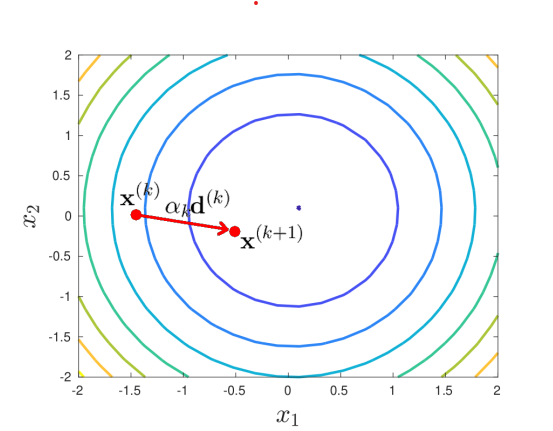
\includegraphics[width=0.5\textwidth]{./img/AnalisiNumerica/gradiente.png}
    \caption{Interpretazione geometrica del metodo del gradiente}
    \label{fig:gradiente}
\end{figure}
Dato che si vuole andare verso il minimo della funzione, l'idea è quella di 
prendere come direzione quella opposta al gradiente. Infatti, il gradiente della 
funzione valutato in un punto restituisce la direzione di massima crescita, la 
direzione opposta corrisponde quindi alla massima decrescita. Fissato $x^{(k)}$,
la direzione di massima decrescita è data da:
\begin{equation}
    d^{(k)} = -\triangledown \phi = b - Ax^{(k)}
\end{equation}
Tale direzione coincide con il residuo al passo $k$, ovvero:
\begin{equation}
    d^{(k)} = r^{(k)} = b - Ax^{(k)}
\end{equation}
Quindi la formula per l'aggiornamento della variabile $x^{(k)}$ diventa:
\begin{equation}
    x^{(k + 1)} = x^{(k)} + \alpha_{k}r^{(k)}
\end{equation}
% ! La parte su come si calcola $\alpha_k$ non è stata fatta a lezione la devo 
% ! aggiungere?